\documentclass[12pt]{beamer}
\usetheme{metropolis}           % Use metropolis theme
\metroset{titleformat=smallcaps}

\usepackage[utf8]{inputenc}
\usepackage[T1]{fontenc}
\usepackage{textcomp}
% \usepackage{amsmath,amsfonts,amssymb}
\usepackage{url}

% disable Navigation at the bottom
\beamertemplatenavigationsymbolsempty

% Cool font
\usepackage{FiraSans}
% \usepackage[sfdefault,light]{FiraSans}
% \usepackage{newtxsf}

% page numbers
% \setbeamertemplate{footline}[frame number]
% \setbeamertemplate{footline}
% \setbeamertemplate{headline}

% style for source code
\usepackage{listings}
\newcommand{\Hilight}{\makebox[0pt][l]{\color{light-gray}\rule[-4pt]{1.0\linewidth}{12pt}}}
\usepackage{color}
\definecolor{light-gray}{gray}{0.80}
  
% use {\mono lorem} to set something in monospace
\newcommand{\mono}[1]{\ttfamily\fontsize{14}{14}\selectfont #1}

% wanna use Metapost?
\makeatletter
\newcommand\@ptsize{12}
\makeatother

\usepackage{mflogo}
\usepackage{emp}
\DeclareGraphicsRule{*}{mps}{*}{}


\title{Disposition 10: Asynchronous Byzantine Agreement}   
\author{Mathias Ravn Tversted} 
\date{\today} 


%===================================
% Async model: What is it about?
    % No clocks, no timeouts, only eventual delivery


% EITHER THIS   
%===================================
% Async broadcast
    % Definition
    % Bracha broadcast

% OR THIS
% Async Byzantine agreement
    % Definition
    % Randomized


\begin{document}

\frame{\titlepage} 

\frame{\frametitle{Table of contents}\tableofcontents} 
%===================================

\section{Asynchronous Model}
    \begin{frame}
        \frametitle{The asynchronous model}
           With the asynchronous model, we have no notion of clocks. 

           We have no timeouts

           We only have eventual delivery of messages. 
    \end{frame}

    \begin{frame}
        \frametitle{The asynchronous model}
        \begin{itemize}
            \item \textbf{Agreement}: All honest parties make the same decision
            \item \textbf{Validity}: Decision made must be sensible in some sensible
            \item \textbf{Termination}: If all parties run the protocol, eventually all honest parties will make a decision
        \end{itemize}
        Additionally, we say that the protocol does not guarantee liveness until all parties start running it, since people can fail arbitrarily long behind. 
    \end{frame}

\styleA
\section{Asynchronous Broadcast}
    \subsection{From signatures}
    \begin{frame}
        \frametitle{Async Broadcast from signatures}
            \begin{itemize}
                \item We build it with ACast and a simple \textit{ToyPKI}
                \item We will use signatures. A broadcaster $P_i$ will ask all parties to sign the message
                \item To broadcast, wait for $n-t$ signatures. 
                \item Receiver outputs only if it has $n-t$ signatures
            \end{itemize}                
        \end{frame}
        \begin{frame}
            \frametitle{Async Broadcast from signatures 2: This Time It's Protocol}
                \begin{itemize}
                    \item \textbf{Request signatures}: To send a message, send it on ACast. We ask that $n-t$ sign that message.
                    \item \textbf{Grant signatures}: When receiving a message, add your signature to it and send it back to the receiver (on the flooding network)
                    \item \textbf{Collect signatures}: The sender collects $n-t$ signatures. 
                    \item \textbf{Send signatures}:  When sender has collected $n-t$ signatures, broadcast it. When reciving a message signed by $n-t$, output it. 
                \end{itemize}
        \end{frame}


    \begin{frame}
        \frametitle{Agreement}
            If two honest $P_j, P_k$ output $m_j, m_k$, then we want $m_j = m_k$. If there are $t$ corrupted (possibly including sender $P_i$) then we have the following argument: 
            Each party sees $n - t$ distinct signatures. If all corrupt $t$ parties sign both $m_j, m_k$ (causing them to be output), this gives us at most $2t$ signatures. This gives us a total of $(n -t) + 2t = n+t$ distinct signatures on either $m_j$ or $m_k$. 
    \end{frame}

    \begin{frame}
        \frametitle{Validity}
            Honest parties output $m$ from $P_i$ if it sees at least $n -t$ signatures. But then it saw at least $(n-t) - t = t + 1$ signatures from honest parties. But then $t + 1 \geq 1$ honest parties signed $m$. And honest parties only sign the $m$ that comes from $P_i$.
    \end{frame}

    \begin{frame}
        \frametitle{Termination}
            If $P_i$ is honest, it asks all honest parties to sign $m$. At least $n-t$ honest grant signatures. $P_i$ at some point receives $n-t$ signatures on $m$. it then forwards them so all honest $P_j$ receives $m$ with $n-t$ signatures, and so they output $m$.
    \end{frame}

    \subsection{Bracha Broadcast}
        \begin{frame}
            \frametitle{Async Broadcast from Authenticated Channels}
                Actually implementing it with an authenticated channel can be done with Bracha broadcast. It goes as follows:
                Assume $P_1$ is the broadcaster. 
                \begin{itemize}
                    \item $P_1$ gets input $(P_1, bid, m)$ on $ACast_i$ to start. We say it got $(Broadcast, P_1, bid, m)$
                    \item When party outputs $P_n, bid, m$ on $ACast_j$ we say it has output $(Deliver, P_n, bid, m)$
                    \item There are no rounds, only activation rules
                \end{itemize}
        \end{frame}

    \begin{frame}
        \frametitle{Bracha Broadcast}
            \textbf{Send}: $P_1$: On input (BROADCAST, $P_1$, bid, $m$), send (SEND, $P_1$, bid, $m$) to all parties


            \textbf{Echo}: $P_i$: On message (SEND, $P_1$, bid, $m$) from $P_1$, send (ECHO, $P_1$, bid, $m$)


            \textbf{Ready 1}: $P_i$ once message (ECHO, $P_1$, bid, $m$) has been received from $n -t$ parties, send (READY, $P_1$, bid, $m$)
    \end{frame}

    \begin{frame}
        \frametitle{Bracha Broadcast}
            \textbf{Ready 2}: $P_i$ once message (READY, $P_1$, bid, $m$) has been received from $t+1$ parties, send (READY, $P_1$, bid, $m$) to all parties if not yet done


            \textbf{Deliver}: Once message (READY, $P_1$, bid, $m$), has been received from $n-t$ parties, output (DELIVER, $P_1$, bid, $m$) and terminate the protocol
    \end{frame}
    \begin{frame}
        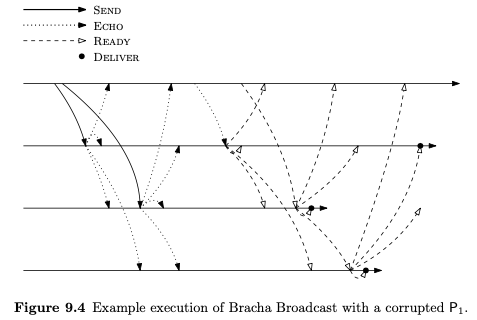
\includegraphics[width=\textwidth]{content/bracha.png}
    \end{frame}
    \begin{frame}
        \frametitle{About Bracha broadcast}
            Each of the preceding rules are activation rules. There are no rounds. The rules can be activated in any order (READY 2 before READY 1 for example). 
            
            We also wait for $n-t$ messages, and not $n$ messages, because we cannot distinguish between late and never arriving messages. When we have enough information we act. 

            If you wait for $t+1$ parties, you are also ensuring you hear from one correct party. We use this to learn that someone honest saw the  mesage $m$. 

            We also need $n > 3t$ to ensure common correct party between two parties. (BEVIS SIDE 210?)
    \end{frame}


\end{document}

